\documentclass[
10pt,reqno
]{amsart}

\usepackage{amsmath}
\usepackage{amssymb}
\usepackage{graphicx}
\usepackage[rightcaption]{sidecap}
\usepackage{amsthm}
\graphicspath{ {../images/} }
\setcounter{section}{4}
\newtheorem{theorem}{Theorem}[section]
\newtheorem{corollary}{Corollary}[section]
\theoremstyle{definition}
\newtheorem{definition}{Definition}[section]

\title{Chapter 4 - Mathematical Expectation}
\setlength{\parindent}{0pt}
\begin{document}
\maketitle


\section*{4.1 Introduction}

\textbf{Mathematical Expectation} - Idea arising from games; the product of the amount a player stands to win and the probability that he or she will win

\section*{4.2 The Expected Value of a Random Variable}

\begin{definition}[Expected Value]
If \(X\) is a discrete random variable and \(f(x)\) is the value of its probability distribution at \(x\), the \textbf{expected value of \(X\)} is
\[
E(X)= \underset{x} \sum x \cdot f(x)
\]
Correspondingly, if \(X\) is a continuous random variable and \(f(x)\) is the value of its probability density at \(x\), the \textbf{expected value of \(X\)} is
\[
E(X)=\int_{- \infty}^{\infty} x \cdot f(x) dx
\]
\end{definition}

\begin{theorem}[Expected Value w/ function of X]
\label{thm:ExpValwFunctionX}
If \(X\) is a discrete random variable and \(f(x)\) is the value of its probability distribution at \(x\), the expected value of \(g(x)\) is given by
\[
E[g(x)]= \underset{x}\sum g(x) \cdot f(x)
\]
Correspondingly, if \(X\) is a continuous random variable and \(f(x)\) is the value of its probability density at \(x\), the expected value of \(g(X)\) is given by
\[
E[g(x)]=\int_{- \infty}^{ \infty } g(x) \cdot f(x) dx
\]
\end{theorem}

\begin{proof}
Since a more general proof is beyond the scope of this text, we shall prove this theorem here only for the case where \(X\) is discrete and has a finite range. Since \(y=g(x)\) does not necessarily define a one-to-one correspondence, suppose that \(g(x)\) takes on the value \(g_i\) when \(x\) takes on the values \(x_{i1},x_{i2},\ldots,x_{in_i}\). Then, the probability that \(g(X)\) will take on the value \(g_i\) is
\[
P[g(X)=g_i] = \sum_{j=1}^{n_i}f(x_{ij})
\]
and if \(g(x)\) takes on the values \(g_1,g_2,\ldots,g_m\), it follows that
\begin{align*}
E[g(X)]&= \sum_{i=1}^m g_i \cdot P[g(X)=g_i]\\
&= \sum_{i=1}^m g_i \cdot \sum_{j=1}^{n_i} f(x_{ij})\\
&= \sum_{i=1}^m \sum_{j=1}^{n_i} g_i \cdot f(x_{ij})\\
&= \sum_{x} g(x) \cdot f(x)\\
\end{align*}
where the summation extends over all values of \(X\).
\end{proof}

\begin{theorem}[Expected Value coefficient and sum of constants]
If \(a\) and \(b\) are constants, then 
\[
E(aX + b)=aE(X)+b
\]
\end{theorem}

\begin{proof}
Using Theorem~\ref{thm:ExpValwFunctionX} with \(g(X)=aX+b\), we get
\begin{align*}
E(aX+b)&=\int_{-\infty}^{\infty}(ax+b) \cdot f(x) dx\\
&=a \int_{-\infty}^{\infty}x \cdot f(x)dx+b \int_{-\infty}^{\infty}f(x)dx\\
&=aE(X)+b
\end{align*}
\end{proof}

\begin{corollary}
If \(a\) is a constant, then
\[
E(aX)=aE(X)
\]
\end{corollary}

\begin{corollary}
If \(b\) is a constant, then
\[
E(b)=b
\]
\end{corollary}

\begin{theorem}[Expected values for Summation]
If \(c_1, c_2, \ldots , c_n\) are constants, then 
\[
E \left [ \sum_{i=1}^n c_i g_i(X) \right ] = \sum_{i=1}^n c_i E[g_i(X)]
\]
\end{theorem}

\begin{proof}
According to Theorem ~\ref{thm:ExpValwFunctionX} with \(g(X)=\sum_{i=1}^{n} c_i g_i (X)\), we get
\begin{align*}
E \left [ \sum_{i=1}^n c_i g_i(X) \right ] &= \sum_x \left [ \sum_{i=1}^n c_i g_i(x) \right ] f(x)\\
&= \sum_{i=1}^n \sum_x c_i g_i(x)f(x)\\
&= \sum_{i=1}^n c_i \sum_x g_i(x)f(x)\\
&= \sum_{i=1}^n c_i E[g_i(X) ] \\
\end{align*}
\end{proof}

\begin{theorem}[Expected Value for Joint Probability]
If \(X\) and \(Y\) are discrete random variables and \(f(x,y)\) is the value of their joint probability distribution at \((x,y)\), the expected value of \(g(X,Y)\) is
\[
E[g(X,Y)] = \sum_x \sum_y g(x,y) \cdot f(x,y)
\]
Correspondingly, if \(X\) and \(Y\) are continuous random variables and \(f(x,y)\) is the value of their joint probability density at \((x,y)\), the expected value of \(g(X,Y)\) is
\[
E[g(x,y)] = \int_{-\infty}^{\infty} \int_{-\infty}^{\infty} g(x,y) f(x,y) dx dy
\]
\end{theorem}

\begin{theorem}[Expected values for Summation (multiple random variables)]
\label{thm:ExpectedValuesSumMultRV}
If \(c_1, c_2, \ldots , c_n\) are constants, then 
\[
E \left [ \sum_{i=1}^n c_i g_i (X_1, X_2, \ldots, X_k)\right ] = \sum_{i=1}^n c_i E[g_i(X_1, X_2, \ldots, X_k)]
\]
\end{theorem}

\section*{4.3 Moments}

\begin{definition}[Moments About the Origin]
The \textbf{\(r\)th moment about the origin} of a random variable \(X\), denoted by \(\mu_r^{'}\), is the expected value of \(X^{'}\); symbolically
\[
\mu_r^{'} = E(X^r)=\sum_x x^r \cdot f(x)
\]
for \(r=0,1,2,\ldots\) when \(X\) is discrete, and
\[
\mu_r^{'}=E(X^r)=\int_{- \infty}^{\infty} x^r \cdot f(x) dx
\]
when \(X\) is continuous.
\end{definition}

\begin{definition}[Mean of a Distribution]
\(\mu_1^{'}\) is called the \textbf{mean} of the distribution of \(X\), or simply the \textbf{mean of \(X\)}, and it is denoted simply by \(\mu\).
\end{definition}

\begin{definition}[Moments about the Mean]
\label{dfn:MomentsAboutMean}
The \textbf{\(r\)th moment about the mean} of a random variable \(X\), denoted by \(\mu_r\), is the expected value of \((X-\mu)^r\), symbolically
\[
\mu_r = E[(X-\mu)^r]=\sum_x (x-\mu)^r \cdot f(x)
\]
for \(r=0,1,2,\ldots\) when \(X\) is discrete, and
\[
\mu_r=E[(X-\mu)^r]=\int_{- \infty}^{\infty} (x-\mu)^r \cdot f(x) dx
\]
when \(X\) is continuous.
\end{definition}

\begin{definition}[Variance]
\label{dfn:Variance}
\(\mu_2\) is called the \textbf{variance} of the distribution of \(X\), or simply the \textbf{variance of \(X\)}, and is denoted by \(\sigma^2, \, \sigma_x^2, \, var(X)\) or \(V(X)\). The positive square root of the variance, \(\sigma\), is call the \textbf{standard deviation of \(X\)}.
\end{definition}

\begin{theorem}[Variance]
\[
\sigma^2 = \mu_2^{'}-\mu^2
\]
\end{theorem}

\begin{proof}
\begin{align*}
\sigma^2 &= E[(X-\mu)^2]\\
&=E(X^2-2 \mu X+\mu^2)\\
&=E(X^2)-2 \mu E(X)+E(\mu^2)\\
&=E(X^2)-2 \mu \cdot \mu+\mu^2\\
&= \mu_2'-\mu^2
\end{align*}
\end{proof}

\begin{theorem}[Coefficients and sums for variance]
If \(X\) has the variance \(\sigma^2\), then
\[
\text{var}(aX+b)= a^2 \sigma^2
\]
\end{theorem}

\begin{proof}
TBD
\end{proof}

\section*{4.4 Chebyshev's Theorem}

\begin{theorem}[Chebyshev's Theorem]
If \(\mu\) and \(\sigma\) are the mean and the standard deviation of a random variable \(X\), then for any positive constant \(k\) the probability is \emph{at least} \(1 - \frac{1}{k^2}\) that \(X\) will take on a value within \(k\) standard deviationes fo the mean; symbolically,
\[
P(|x-\mu|< k \sigma) \ge 1- \frac{1}{k^2}, \; \sigma \ne 0
\]
\end{theorem}

\begin{proof}
According to Definition ~\ref{dfn:MomentsAboutMean} and Definition ~\ref{dfn:Variance}, we write
\[
\sigma^2 = E[(X-\mu)^2] = \int_{-\infty}^{\infty}(x-\mu)^2 \cdot f(x) dx
\]
\begin{figure}[h]
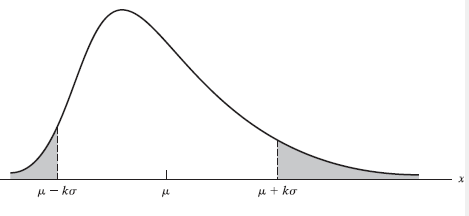
\includegraphics[width=1\textwidth]{ChebyshevsTheorem}
\caption{Diagram for proof of Chebyshev's Theorem}
\label{fig:Chebyshev}
\end{figure}

Then, dividing the integral into three parts as shown in Figure ~\ref{fig:Chebyshev}, we get
\[
\sigma^2 = \int_{- \infty}^{\mu - k \sigma}(x - \mu)^2 \cdot f(x) dx +
\int_{\mu - k \sigma}^{\mu + k \sigma}(x - \mu)^2 \cdot f(x) dx +
\int_{\mu + k \sigma}^{\infty}(x - \mu)^2 \cdot f(x) dx
\]
Since the integrand \((x - \mu)^2 \cdot f(x) \) is nonnegative, we can form the inequality
\[
\sigma^2 \ge \int_{- \infty}^{\mu - k \sigma}(x - \mu)^2 \cdot f(x) dx +
\int_{\mu + k \sigma}^{\infty}(x - \mu)^2 \cdot f(x) dx
\]
by deleting the second integral. Therefore, since \((x-\mu)^2 \ge k^2 \sigma ^2\) for \(x \le \mu - k\sigma \) or \(x \ge \mu + k \sigma \) it follows that
\[
\sigma^2 \ge \int_{- \infty}^{\mu - k \sigma} k^2 \sigma^2 \cdot f(x) dx +
\int_{\mu + k \sigma}^{\infty}k^2 \sigma^2 \cdot f(x) dx
\]
and hence that
\[
\frac{1}{k^2} \ge \int_{- \infty}^{\mu -k \sigma} f(x) dx +
\int_{\mu + k \sigma}^{\infty} f(x) dx
\]
provided \(\sigma^2 \ne 0\). Since the sum of the two integrals on the right-hand side is the probability that \(X\) will take on a value less than or equal to \(\mu - k \sigma \) or greater than or equal to \( \mu +k \sigma\), we have thus shown that 
\[
P(|X-\mu| \ge k \sigma) \le \frac{1}{k^2}
\]
and it follows that
\[
P(|X-\mu| < k \sigma) \ge 1 - \frac{1}{k^2}
\]
\end{proof}

\newpage

\section*{4.5 Moment-Generating Function}

\begin{definition}
The \textbf{moment generating function} of a random variable \(X\), where it exists, is given by
\[
M_X(t)= E(e^{tX}) = \sum_x e^{tX} \cdot f(x)
\]
when \(X\) is discrete, and 
\[
M_X(t)= E(e^{tX}) = \int_{- \infty}^{\infty}e^{tx} \cdot f(x) dx
\]
when \(X\) is continuous.
\end{definition}

\begin{theorem}[Derivative of Moment Generating Function]
\[
\frac{d^r M_X(t)}{dt^r} \Bigg \vert _{t=0}=\mu_r^{'}
\]
\end{theorem}

\begin{theorem}
If \(a\) and \(b\) are constants, then:
\begin{enumerate}
	\item \( M_{X+a}(t) = E [e^{(X + a)t}] = e^{at} \cdot M_X (t)\)
	\item \( M_{bX}(t) = E (e^{bXt}) = M_X (bt)\)
	\item \( M_{\frac{X+a}{b}}(t) = E [e^{(\frac{X + a}{b})t}] = e^{\frac{a}{b}t} \cdot M_X (\frac{t}{b})\)
\end{enumerate}
\end{theorem}

\begin{proof}
TBD Exercise 4.39
\end{proof}

\section*{4.6 Product Moments}

\begin{definition}[Product Moments About the Origin]
The \textbf{\(r\)th and \(s\)th product moment about the origin} of the random variables \(X\) and \(Y\), denoted by \(\mu^{'}_{r,s}\), is the expected value of \(X^r Y^s\); symbolically,
\[
\mu^{'}_{r,s}= E(X^r Y^s)=\sum_x \sum_y x^r y^s \cdot f(x,y)
\]
for \(r=0,1,2, \ldots \) and \(s=0,1,2,\ldots\) when \(X\) and \(Y\) are discrete, and
\[
\mu^{'}_{r,s}= E(X^r Y^s)=\int_{- \infty}^{\infty} \int_{- \infty}^{\infty} x^r y^s \cdot f(x,y) dx dy
\]
when \(X\) and \(Y\) are continuous.
\end{definition}

\begin{definition}
The \textbf{\(r\)th and \(s\)th product moment about the means} of the random variables \(X\) and \(Y\), denoted by \(\mu_{r,s}\), is the expected value of \((X-\mu_X)^r (Y - \mu_Y)^s\); symbolically,
\begin{align*}
\mu_{r,s} &= E[(X- \mu_X)^r (Y - \mu_Y)^s)]\\
&=\sum_x \sum_y (x - \mu_X)^r (y - \mu_Y)^s \cdot f(x,y)
\end{align*}
for \(r=0,1,2, \ldots \) and \(s=0,1,2,\ldots\) when \(X\) and \(Y\) are discrete, and
\begin{align*}
\mu_{r,s} &= E[(X- \mu_X)^r (Y - \mu_Y)^s)]\\
&= \int_{- \infty}^{\infty} \int_{- \infty}^{\infty} (x - \mu_X)^r (y - \mu_Y)^s \cdot f(x,y)
\end{align*}
when \(X\) and \(Y\) are continuous.
\end{definition}

\begin{definition}[Covariance]
\(\mu_{1,1}\) is called the \textbf{covaraince} of \(X\) and \(Y\), and it is denoted by \(\sigma_{XY}\), cov(\(X,Y\)), or C(\(X,Y\))
\end{definition}

\begin{theorem}
\[
\sigma_{XY} = \mu_{1,1}^{'}-\mu_{X} \mu_{Y}
\]
\end{theorem}

\begin{proof}
Using the various theorems about expected values, we can write
\begin{align*}
\sigma_{XY} &= E[(X-\mu_X)(Y-\mu_Y)]\\
&=E(XY-X \mu_Y - Y \mu_X - \mu_X \mu_Y)\\
&=E(XY) - \mu_Y E(X)-\mu_X E(Y) +\mu_X \mu_Y\\
&=E(XY) - \mu_Y \mu_X-\mu_X \mu_Y  +\mu_X \mu_Y\\
&=\mu_{1,1}^{'}-\mu_{X} \mu_{Y}\\
\end{align*}
\end{proof}

\begin{theorem}
If \(X\) and \(Y\) are independent, then \(E(XY)= E(X) \cdot E(Y)\) and \(\sigma_{XY} =0 \)
\end{theorem}
\begin{proof}
For the discrete case we have, by definiteion, 
\[
E(XY)=\sum_x \sum_y xy \cdot f(x,y)
\]
Since \(X\) and \(Y\) are independent, we can write \(f(x,y)=g(x)\cdot h(y)\), where \(g(x)\) and \(h(y)\) are the values of the marginal distributions of \(X\) and \(Y\), and we get
\begin{align*}
E(XY)&=\sum_x \sum_y xy \cdot g(x) h(y)\\
&=\left [ \sum_x x \cdot g(x) \right ]\left [ \sum_y y \cdot h(y) \right ]\\
&= E(X) \cdot E(Y)
\end{align*}
Hence,
\begin{align*}
\sigma_{XY} &= \mu_{1,1}^{'}-\mu_{X} \mu_{Y}\\
&=E(X) \cdot E(Y) - E(X) \cdot E(Y)\\
&=0
\end{align*}
\end{proof}

\begin{theorem}
If \(X_1, X_2,\ldots,X_n\) are independent, then 
\[
E(X_1, X_2,\ldots,X_n)=E(X_1)\cdot E(X_2) \cdot \ldots \cdot E(X_n)
\]
\end{theorem}

\newpage

\section*{4.7 Moments of Linear Combinations of Random Variables}

\begin{theorem}
If \(X_1, X_2,\ldots,X_n\) are random variables and 
\[
Y = \sum_{i=1}^n a_i X_i
\]
where \(a_1, a_2, \ldots, a_n\) are constants, then 
\[
E(Y) = \sum_{i=1}^n a_i E(X_i)
\]
and
\[
\text{var}(Y)=\sum_{i=1}^n a_i^2 \cdot \text{var}(X_i)+ 2 \underset{i < j}{\sum \sum} a_i a_j \cdot \text{cov} (X_i X_j)
\]
where the double summation extends over all values of \(i\) and \(j\), from 1 to \(n\), for which \(i < j\).
\end{theorem}

\begin{proof}
From Theorem ~\ref{thm:ExpectedValuesSumMultRV} with \(g_i (X_1, X_2, \ldots, X_k)=X_i\) for \(i=0,1,2, \ldots n \) it follows that immediately that
\[
E(Y)=E \left ( \sum_{i=1}^n a_iX_i \right ) = \sum_{i=1}^n a_i E(X_i)
\]
and this proves the first part of the theorem. To obtain the expression for the variance of \(Y\), let us write \( \mu_i \) for \(E(X_i)\) so that we get
\begin{align*}
\text{var}(Y) = E([Y-E(Y)]^2)&=E \left \{  \left [ \sum_{i=1}^n a_i X_i  - \sum_{i=1}^n a_i E(X_i)\right ]^2 \right \}\\
&=E \left \{  \left [ \sum_{i=1}^n a_i (X_i  - \mu_i)\right ]^2 \right \}
\end{align*}
Then, expanding by means of the multinomial theorem, according to which \((a+b+c+d)^2\), for example, equals \(a^2+b^2+c^c+d^2+2ab+2ac+2ad+2bc+2bd+2cd\), and again referring to Theorem ~\ref{thm:ExpectedValuesSumMultRV}, we get
\begin{align*}
\text{var}(Y) &= \sum_{i=1}^n a_i^2 E[(X_i - \mu_i)^2]+ 2 \underset{i<j}{\sum \sum}a_i a_j E[(X_i - \mu_i)(X_j - \mu_j)]\\
&= \sum_{i=1}^n a_i^2 \cdot \text{var} (X_i)+ 2 \underset{i<j}{\sum \sum}a_i a_j \cdot \text{cov}(X_i,X_j)\\
\end{align*}
Note that we have tacitly made use of the fact that \(\text{cov}(X_i, X_j)=\text{cov}(X_j,X_i)\)
\end{proof}

\begin{corollary}
If the random variables \(X_1, X_2,\ldots,X_n\) are independent and \(Y=\sum_{i=1}^n a_i X_i\), then
\[
\text{var}(Y)=\sum_{i=1}^n a_i^2 \cdot \text{var}(X_i)
\]
\end{corollary}

\begin{theorem}
If \(X_1, X_2,\ldots,X_n\) are random variables and
\begin{align*}
Y_1=\sum_{i=1}^n a_i X_i \; \text{and} \; Y_2=\sum_{i=1}^n b_i X_i
\end{align*}
where \(a_1,a_2,\ldots,a_n,b_1, b_2, \ldots, b_n\) are constants, then
\begin{align*}
\text{cov}(Y_1,Y_2) = \sum_{i=1}^n a_i b_i \cdot \text{var} (X_i)+ \underset{i<j}{\sum \sum}(a_i b_j + a_j b_i) \cdot \text{cov}(X_i,X_j)\\
\end{align*}
\end{theorem}

\begin{corollary}
If the random variables \(X_1, X_2,\ldots,X_n\) are independent, \(Y_1=\sum_{i=1}^n a_i X_i\) and \(Y_2=\sum_{i=1}^n b_i X_i\)
\[
\text{cov}(Y_1, Y_2)=\sum_{i=1}^n a_i b_i \cdot \text{var}(X_i)
\]
\end{corollary}

\section*{4.8 Conditional Expectations}

\begin{definition}
If \(X\) is a discrete random variable, and \(f(x|y)\) is the value of the conditional probability distribution of \(X\) give \(Y=y\) at \(x\), the \textbf{conditional expectation of \(u(X)\) given \(Y=y\)} is
\[
E[(u(X)|y)]=\sum_x u(x)\cdot f(x|y)
\]
Correspondingly, if \(X\) is a continuous variable and \(f(x|y)\) is the value of the conditional probability distribution of \(X\) given \(Y=y\) at \(x\), the \textbf{conditional expectation of \(u(X)\) given \(Y=y\)} is
\[
E[(u(X)|y)]=\int_{- \infty}^{\infty} u(x)\cdot f(x|y)dx
\]
\end{definition}

\textbf{Conditional Mean}
\[
\mu_{X|y}=E(X|y)
\]

\textbf{Conditional Variance}
of \(X\) given \(Y=y\)
\begin{align*}
\sigma_{X|y}^2&=E[(X - \mu_{X|y})^2|y]\\
&=E(X^2|y)-\mu_{X|y}^2
\end{align*}

\section*{4.9 The Theory in Practice}

\textbf{Sample Mean}
\[
\overline{x}=\sum_{i=1}^n \frac{x_i}{n}
\]

\textbf{Median} Arrange the observations in ascending order:
\begin{itemize}
	\item if the number of observations \(n\) is odd, then the median is the observation at position \(\frac{n+1}{2}\)
	\item if the number of observations \(n\) is even, then the median is the average of the two observations at
  \(\frac{n}{2}\) and \(\frac{n}{2} + 1\)
\end{itemize}

\textbf{Sample Standard Deviation}
\[
s=\sqrt{\frac{\sum_{i=1}^n (x-\overline{x})^2}{n-1}}
\]
but since this requires finding the mean first the following is equivalent, but doesn't require finding the mean
\[
s=\sqrt{\frac{n\sum_{i=1}^n x_i^2-(\sum_{i=1}^n x_i)^2}{n(n-1)}}
\]

\end{document}
